\usepackage{graphicx}\section{Anhang A: UML-Diagramme (vollständig)}
\label{sec:anhang-a}

Dieser Anhang enthält alle vollständigen UML-Diagramme in hoher Auflösung.

\subsection{Klassen-Diagramm}
\begin{figure}[H]
    \centering
    
\includegraphics[width=\textwidth]{../diagrams/class-diagram.png}
    \caption{Vollständiges Klassen-Diagramm}
\end{figure}

\subsection{Komponenten-Diagramm}
\begin{figure}[H]
    \centering
    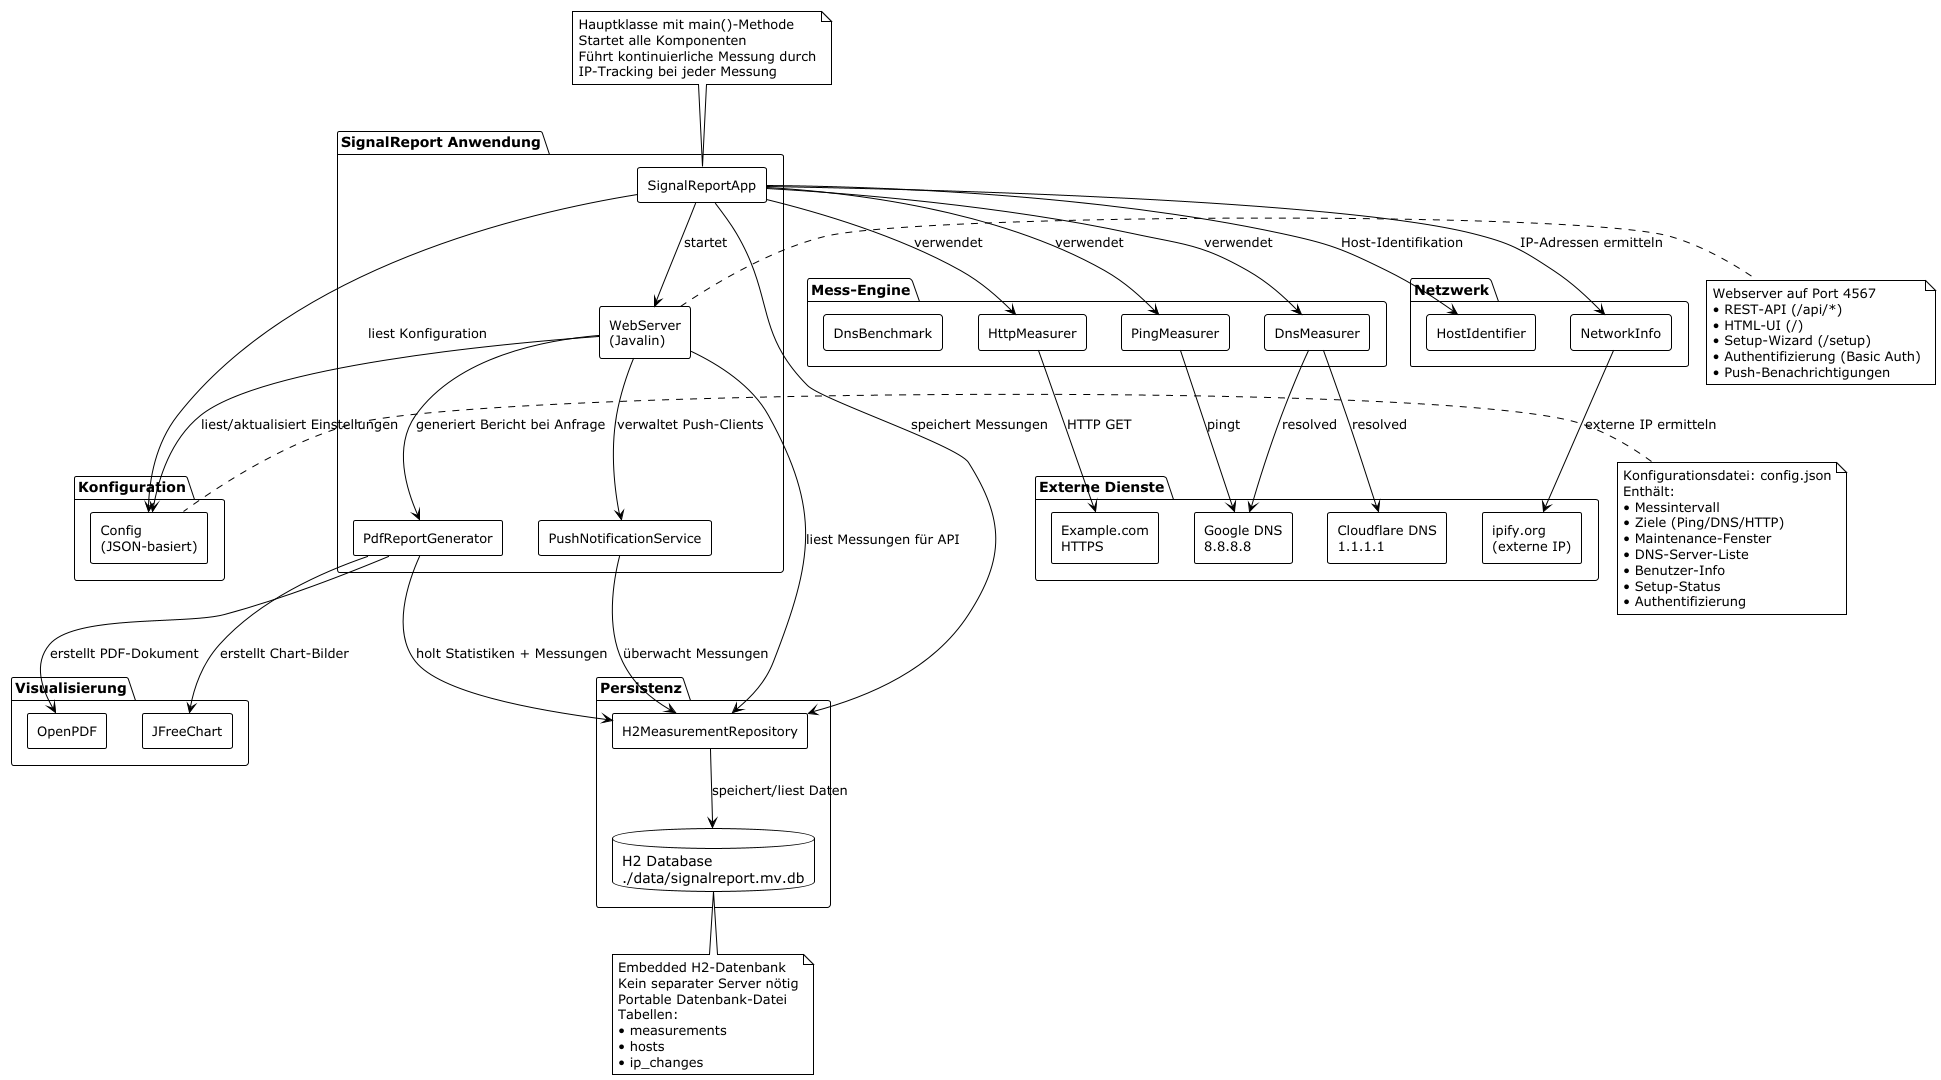
\includegraphics[width=\textwidth]{../diagrams/component-diagram.png}
    \caption{Vollständiges Komponenten-Diagramm}
\end{figure}

\subsection{Sequenz-Diagramm: Messungsablauf}
\begin{figure}[H]
    \centering
    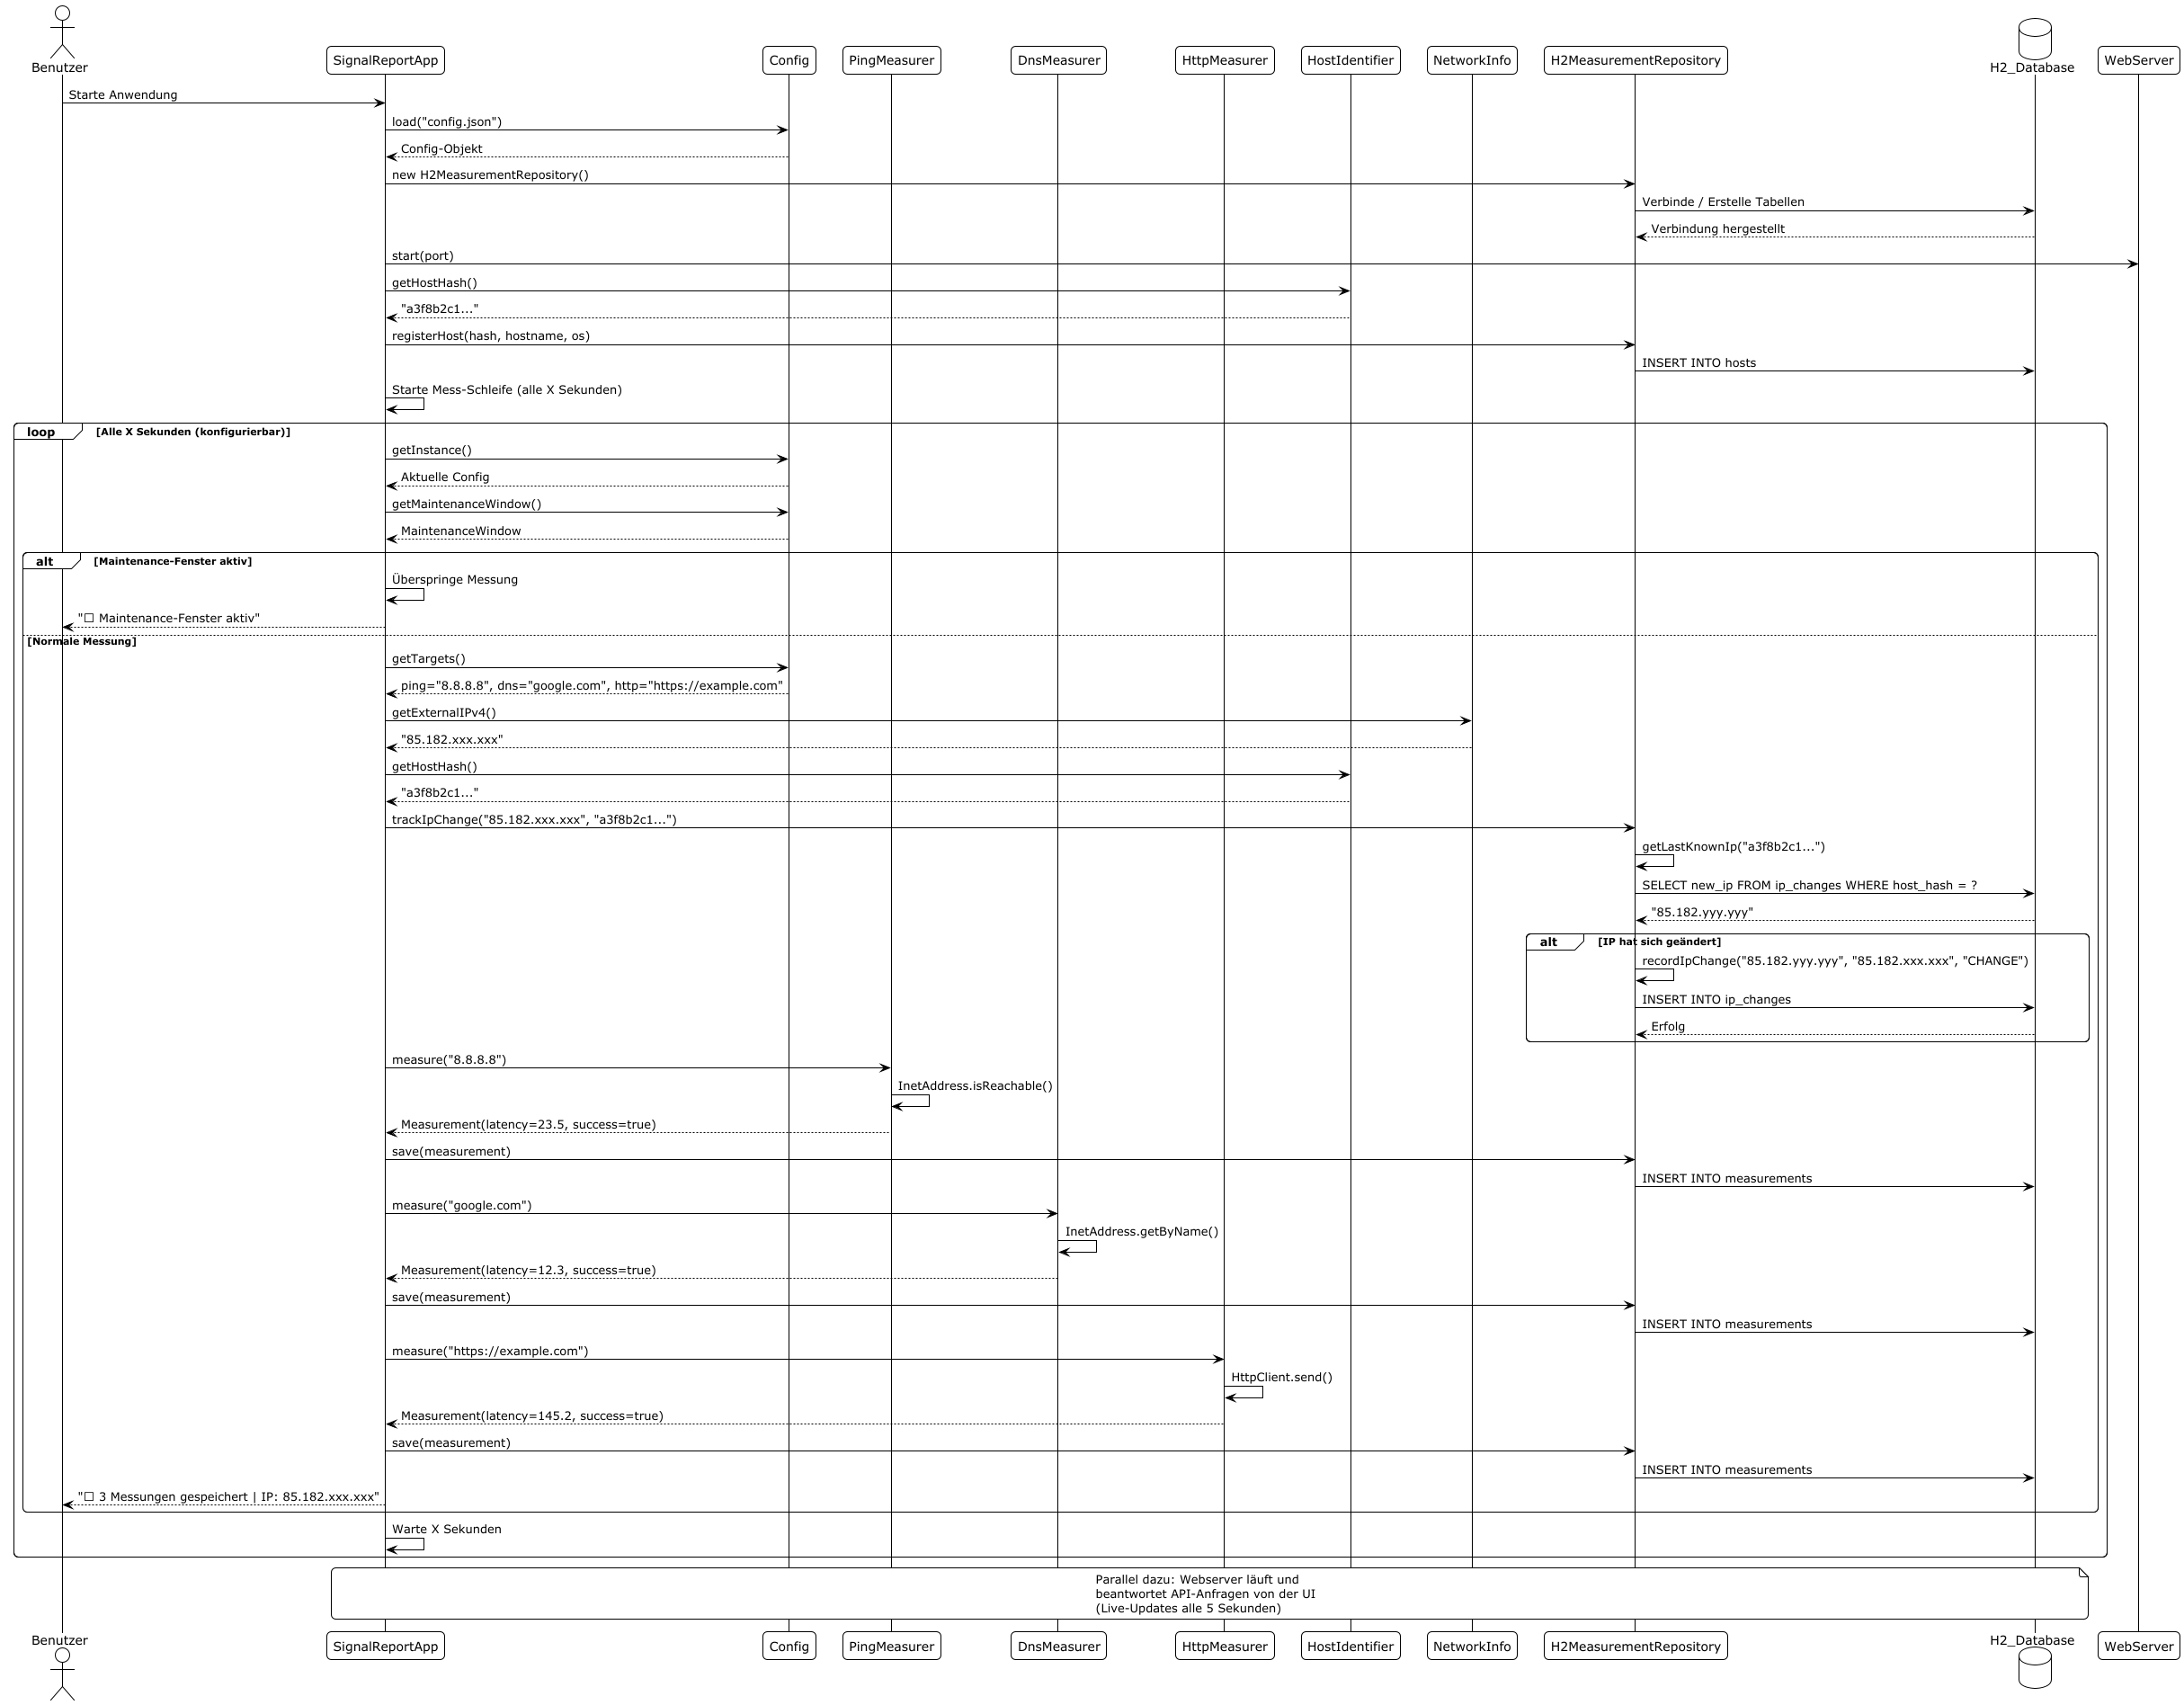
\includegraphics[width=\textwidth]{../diagrams/sequence-measurement.png}
    \caption{Vollständiges Sequenz-Diagramm Messungsablauf}
\end{figure}

\subsection{Sequenz-Diagramm: PDF-Export}
\begin{figure}[H]
    \centering
    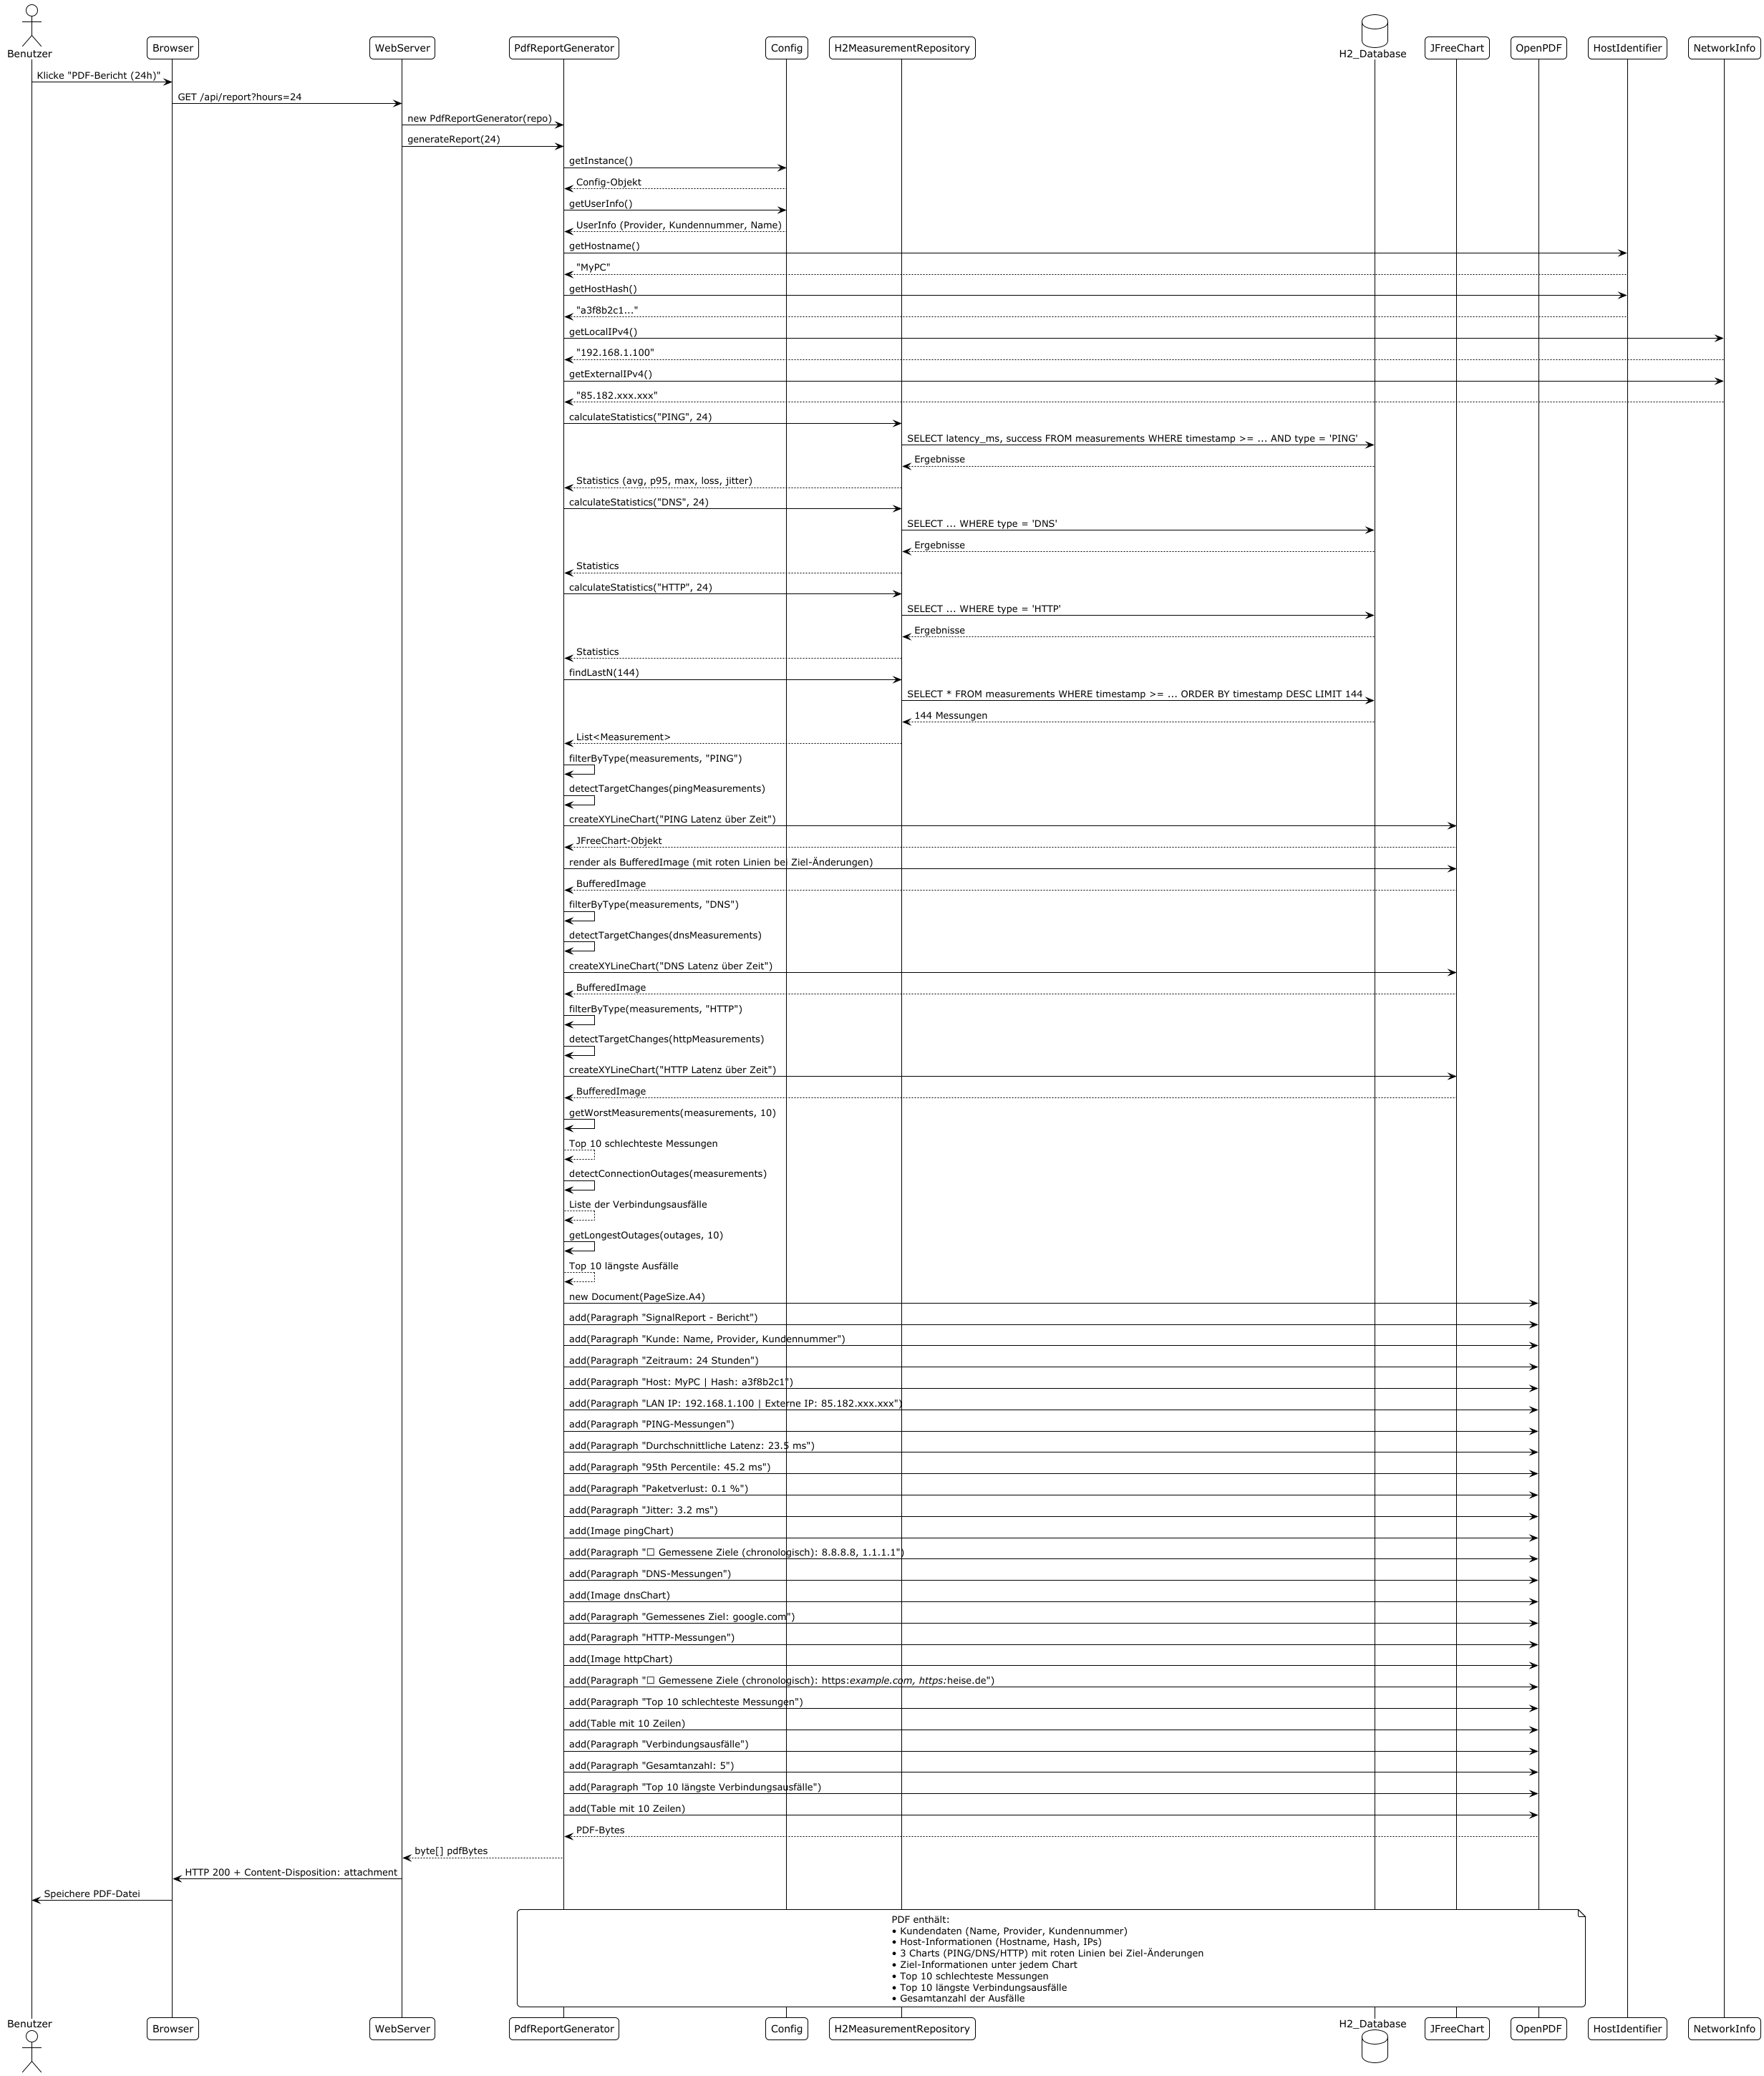
\includegraphics[width=\textwidth]{../diagrams/sequence-pdf.png}
    \caption{Vollständiges Sequenz-Diagramm PDF-Export}
\end{figure}

\subsection{Use-Case-Diagramm}
\begin{figure}[H]
    \centering
    
\includegraphics[width=0.9\textwidth]{../diagrams/usecase-diagram.png}
    \caption{Vollständiges Use-Case-Diagramm}
\end{figure}

\subsection{Deployment-Diagramm}
\begin{figure}[H]
    \centering
    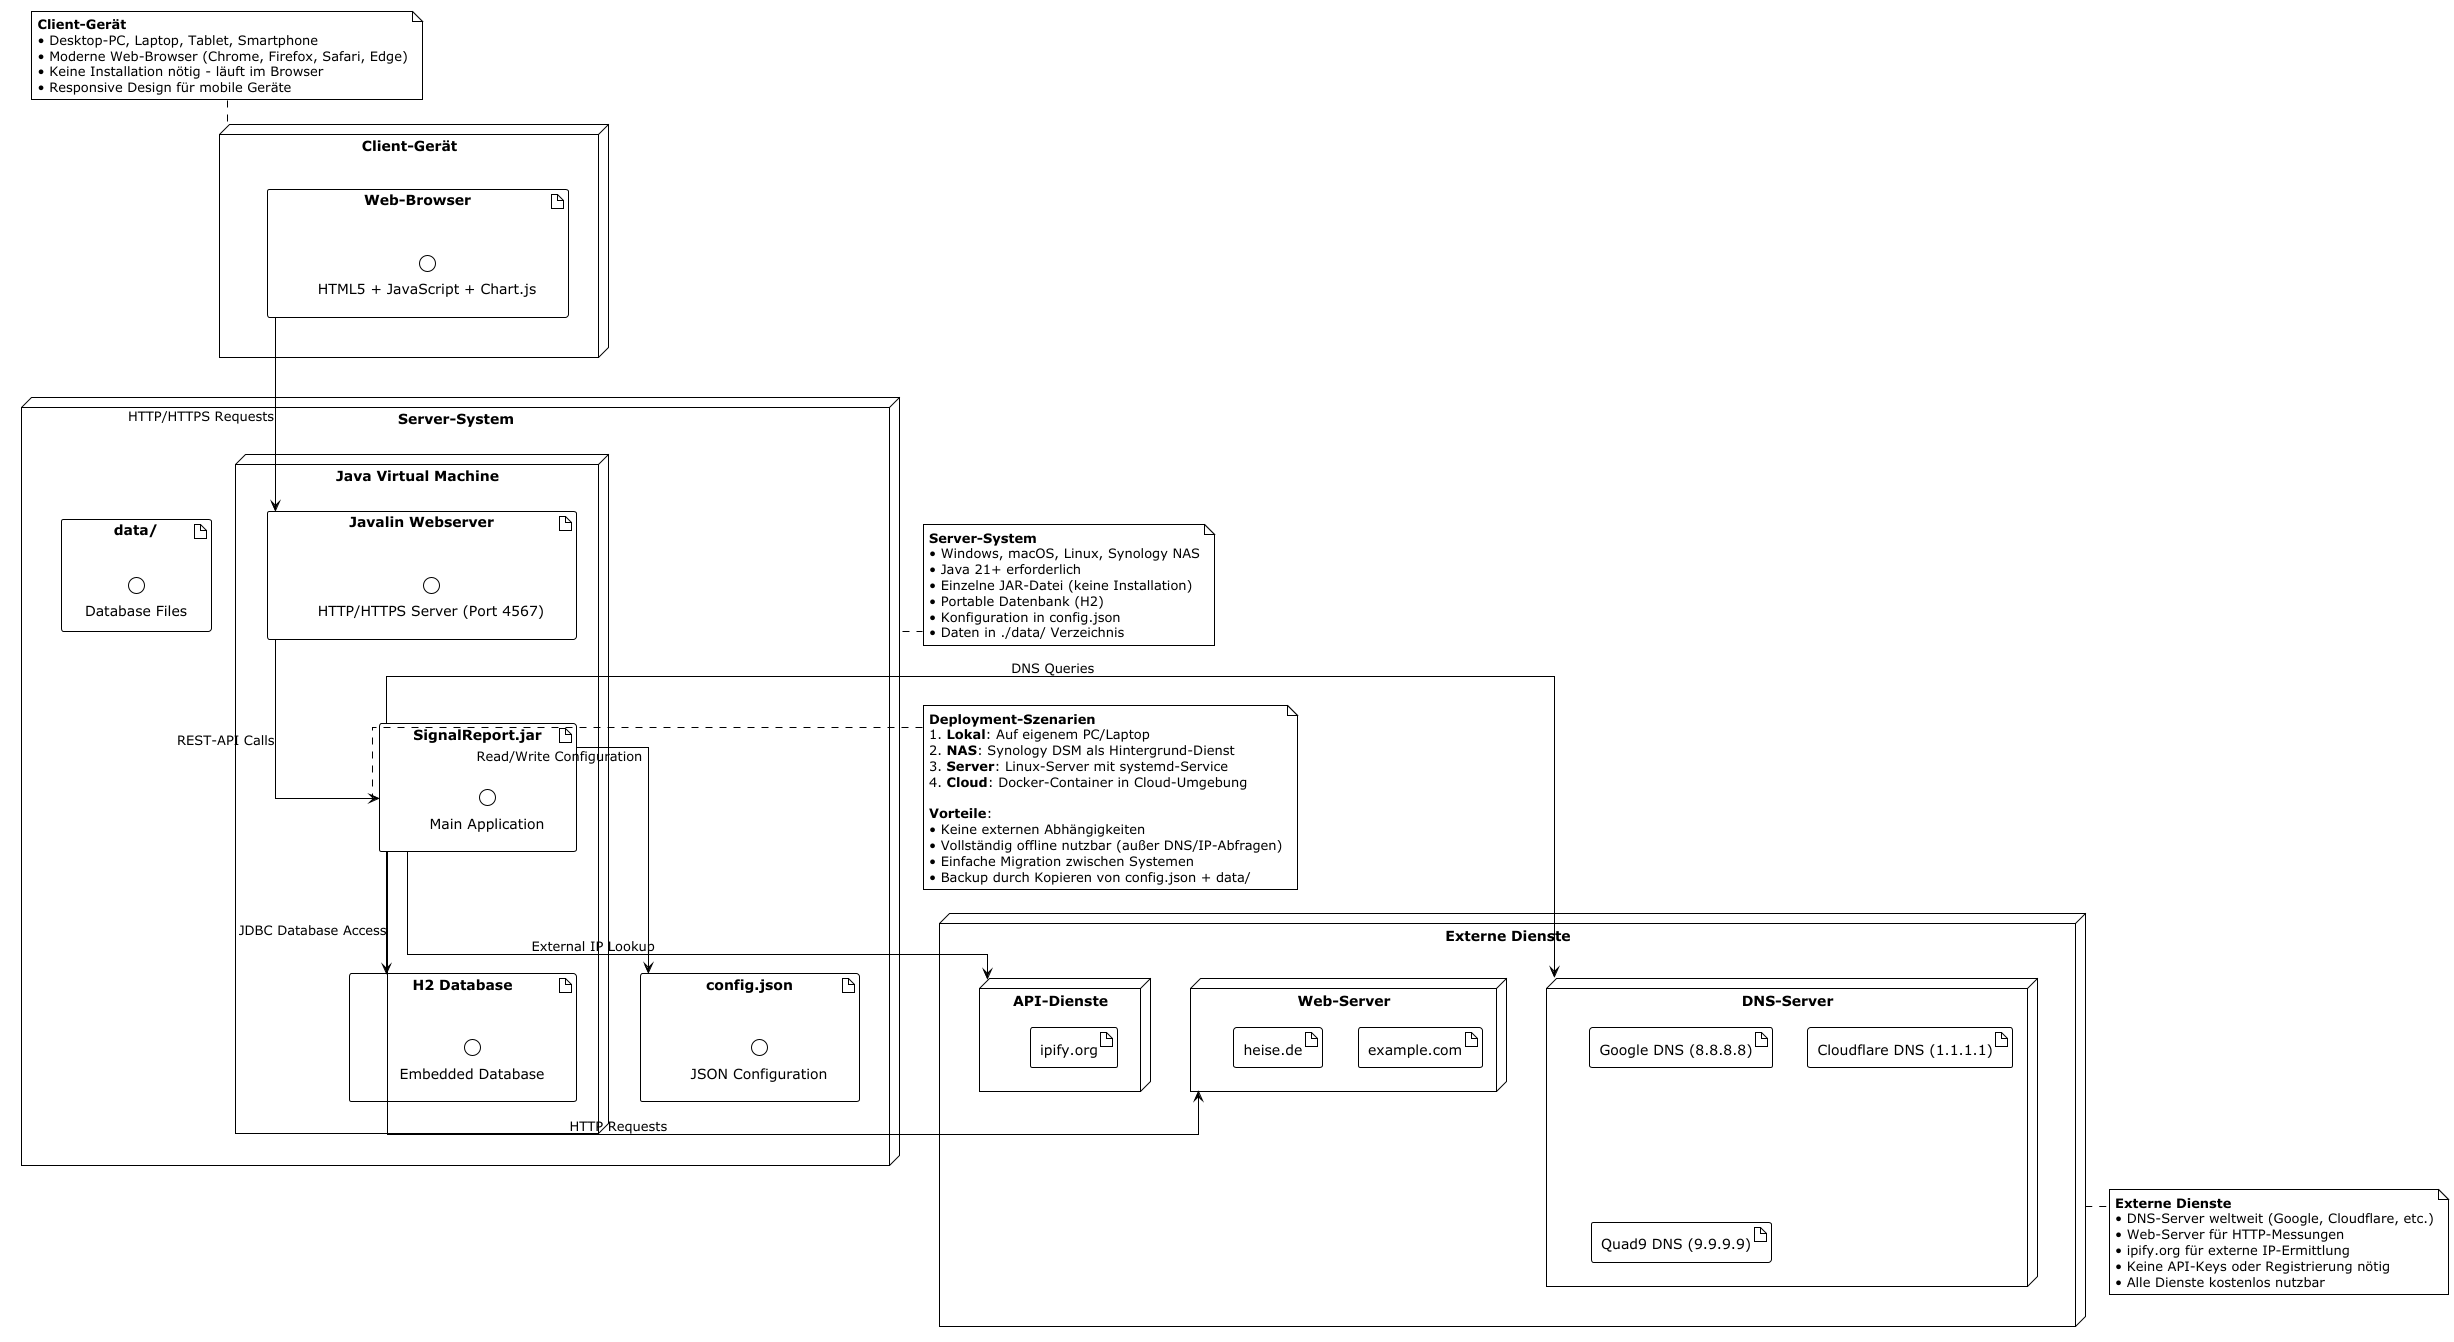
\includegraphics[width=0.9\textwidth]{../diagrams/deployment-diagram.png}
    \caption{Vollständiges Deployment-Diagramm}
\end{figure}

\subsection{State-Diagramm: Authentifizierung}
\begin{figure}[H]
    \centering
    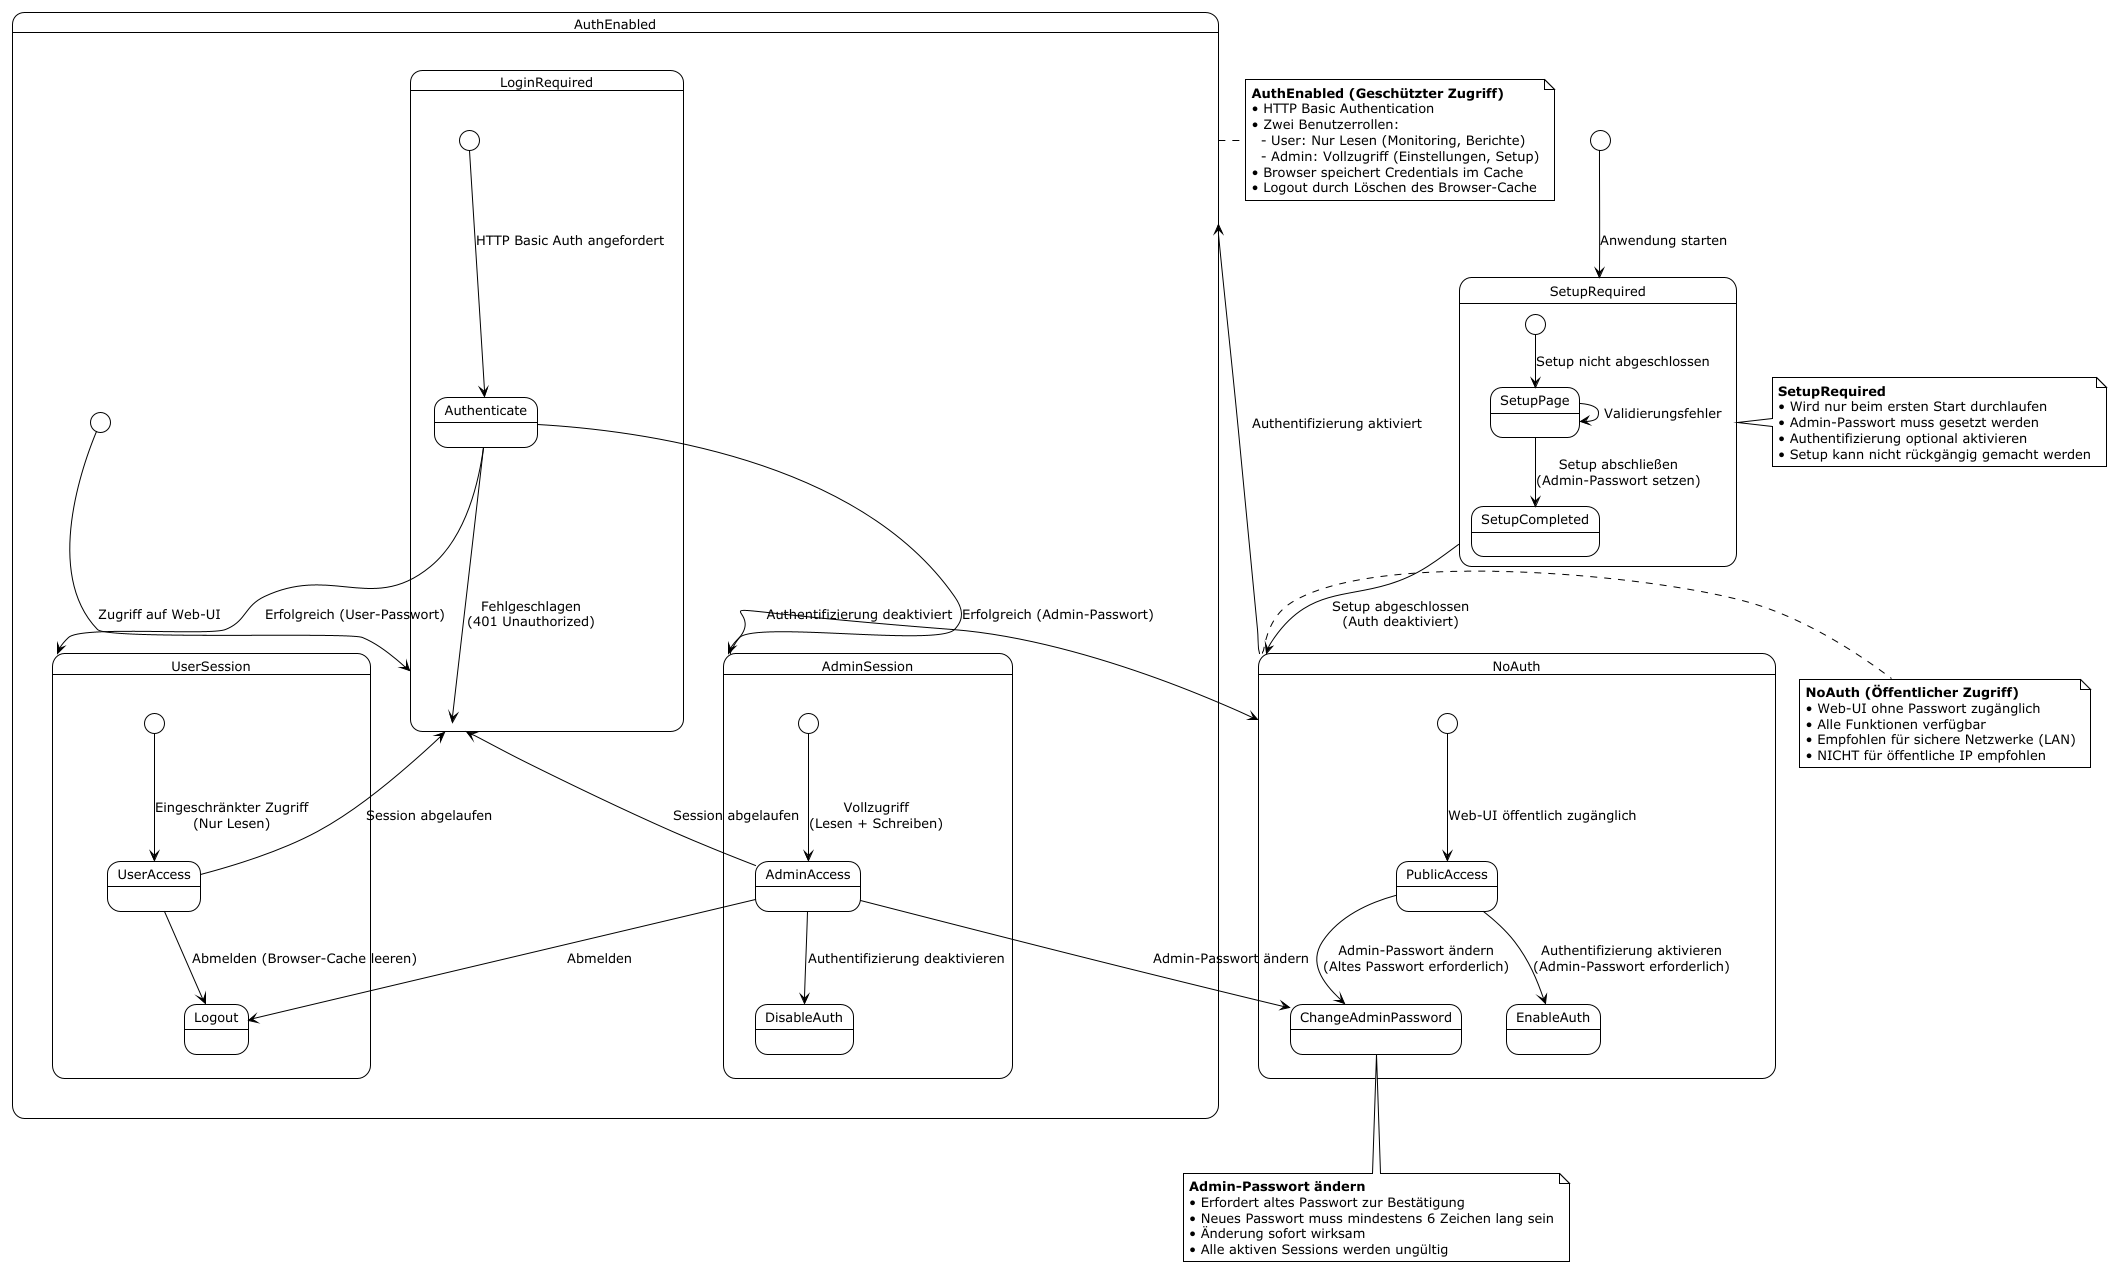
\includegraphics[width=0.9\textwidth]{../diagrams/state-diagram-auth.png}
    \caption{Vollständiges State-Diagramm Authentifizierung}
\end{figure}